\section{Introduction}

Cloud computing has marked significant developments and possibilities in the industry. It focuses on offering services for the different needs of the modern society.


There are three categories of cloud computing services namely, Software as a Service (SaaS), Platform as a Service (PaaS) and Infrastructure as a Service (IaaS). Organizations provide SaaS depending on the demand. Google Apps is one example of SaaS that can be used to manage email and create documents, etc. PaaS offers developers a platform where they can build and deploy applications. IaaS provides storage, servers and clusters. These tools are primarily created to serve computational needs \cite {Ahuja2012}. A cloud computing platform dynamically allocates, configures, reconfigures and deallocates servers as requested or on demand. This approach ensures the elasticity of cloud computing \cite {Brandic2011}.


Most scientific applications require high performance computing (HPC) which needs CPU intensive computations and large data storage. To be able to host such applications, several computers interconnected in a network such as clusters are needed. This makes scientific computing very costly in terms of hardware infrastructure investment. With the advancement in cloud computing, these scientific applications  can be deployed in the cloud without worrying about hardware costs and maintenance \cite {Ahuja2012}. However, studies have shown that network transmission delay is the major drawback in deploying HPC applications in the cloud\cite {Brandic2011}. 

Peak-Two Cloud (P2C) is a private cloud based on OpenStack designed for research in deploying HPC applications in the cloud\cite {Hermocilla2014}. One of the features introduced by P2C is vCluster. vCluster is a tool that enables a user to deploy a working (Message Passing Interface) cluster on demand and to terminate it after use. P2C has been used by researchers in various fields including bioinformatics, quantum chemistry, and molecular dynamics. These researchers belong to different research groups who have little or no investment in HPC infrastructure due to limited funding but requires heavy computing resources for their research. vCluster, however, is a command line application which make it difficult for non-technical users (physicists, chemists, and biologists) to use. A more user-friendly interface is needed in order to enable scientists to focus more on their science rather than on learning and using the command  line.

Presented in this paper is Skylab\footnote{https://github.com/vincentpaul12/SkyLab}, a workflow web application on top of vCluster that addresses the concern above. Specifically, SkyLab will  

\begin{enumerate}
	\item allow users to execute HPC tools via web interface; 
	\item enable developers to easily extend it to support additional HPC tools;
	\item enable users to share their instantiated clusters; and
	\item support displaying of results using third party tools.
\end{enumerate}
   
The following are the tools that are currently supported by SkyLab. They are commonly used by collaborators from different research groups.

\begin{itemize}
    	\item \textit{AutoDock} - A software used to simulate protein-ligand docking\cite{morris2009autodock4}.

        \item \textit{AutoDock Vina} - A software similar to AutoDock 4 but on the average, it provides faster and more accurate computations \cite{JCC:JCC21334}. 
            
		\item \textit{DOCK} - Used to predict the small molecule-target interactions    \cite{lang2009dock}.
            
      	\item \textit{Quantum ESPRESSO} - An integrated software suite of tools for ab-initio molecular dynamics (MD) simulations and electronic structure calculations\cite{QE-2009}.

  		\item \textit{GAMESS} - Used for ab initio molecular quantum chemistry  \cite{1993gamess}.
            
 	    \item \textit{Ray} - Uses parallel genome assemblies for parallel DNA sequencing \cite{boisvert_ray_2012}.
 	    
 	    \item \textit{Impi} - MPI implementation of some image processing routines \cite{trajano2010}. 

\end{itemize}   
      
\section{Design and Implementation}

SkyLab is implemented as a web application (using the Django Web Framework\footnote{https://www.djangoproject.com/}) in order to provide users access to their HPC applications by just using a web browser. This makes it challenging to implement given that multiple tools must be supported. Also, HPC applications executed through SkyLab have their own process space, separate from the process on which SkyLab is running. This makes it diffucult to keep track of the applications and may even pose security threats. 

Figure ~\ref{fig:sysarch} shows the layers on which SkyLab is built on. At the bottom layer is P2C which provides the cloud infrastructure. vCluster is for on-demand provisioning and termination of MPI clusters. p2c-tools is the command line tool for activating the required HPC tool.

	\begin{figure}[h]			
		%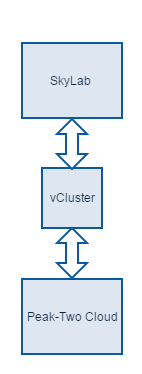
\includegraphics[width=92px,height=224px]{./images/system_architecture.png}	
		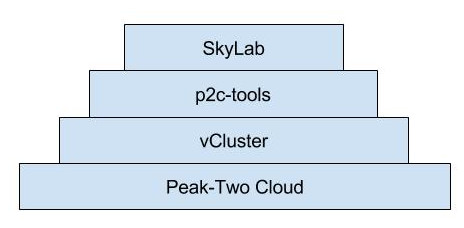
\includegraphics[scale=0.30]{./images/skylab_layers.jpg}			
		\caption{\label{fig:sysarch}Layers on which SkyLab is built on.}	
	\end{figure}	

The use case on which SkyLab was designed is shown in Figure ~\ref{fig:usecase}. Users must first create a cluster then activate the desired tool to use.

    
    \begin{figure*}[ht]
      \centering
      %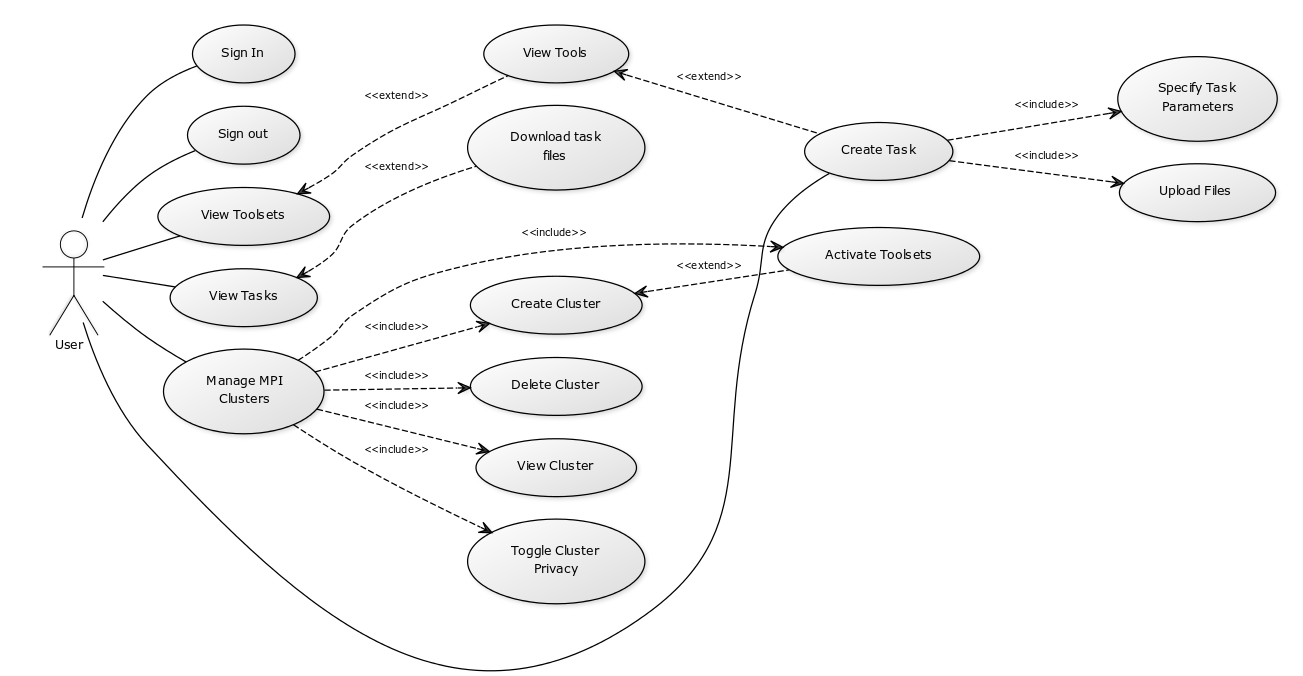
\includegraphics[width=500px,height=250px]{./images/use_case_large.png}
      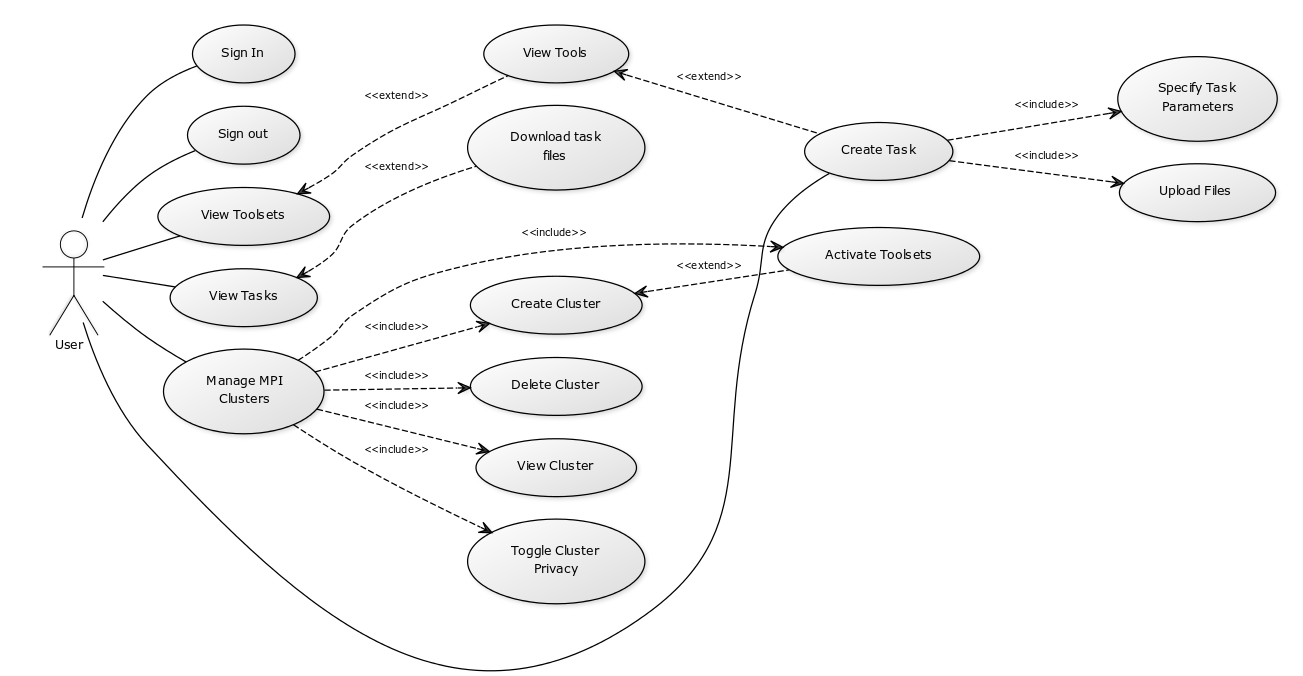
\includegraphics[scale=0.36]{./images/use_case_large.png}
      \caption{\label{fig:usecase}Use Case Diagram}
    \end{figure*}


\subsection{MPI clusters} 

The system spawns a thread (MPIThread) for each active cluster which handles the connection to the assigned cluster via Secure Shell (SSH). Creation and deletion of clusters is done by using vCluster commands while tool activation is done by using p2c-tools. The thread also manages task queuing and execution.
		
A cluster is either classified as public or private. If it is set to public, every user in the system can use it. On the other hand, for private clusters, the cluster will only be visible to the owner. The owner has the option to share the cluster to other users via the share key generated for the said cluster. 		

\subsection{Tool sets} 
The system searches for Python packages inside the assigned modules folder and install it on server start. The tool sets will then be available for use with the system. The package must have a Python module named \emph{install.py} which contains function calls for integrating the package with the system. The package must also contain the corresponding views and executable classes for each sub-tool.  

\subsection{Tasks} 
The system creates a task object for each task input by the user. A signal will then be sent and it is then received by the corresponding MPIThread which queues the task for execution. When a task is executed, it calls the assigned executable class with the given parameters. On connection error, the task waits exponentially before retrying. If the server crashes while running task execution, the task is just restarted.				
		
Default task execution flow via executable class:			
	\begin{enumerate}
		\item  Needed remote and local directories for execution are cleared or created.
		\item  Input files are uploaded to cluster.
		\item  List of commands given are executed.
		\item  Output files are sent back to the server.
		\item  Remote task folder is deleted.
		\item  Output files are served by the server.
	\end{enumerate}	

	
\section{Results and Discussion}


          
\subsection{System Features}
The system's interface offers different functionalities that simplifies MPI cluster and task management.
		
	\begin{itemize}
		\item The user is authenticated by logging in with his @up.edu.ph Google account.
		\item The user can create an MPI cluster with optional tool activations. 
			\begin{center}			
				%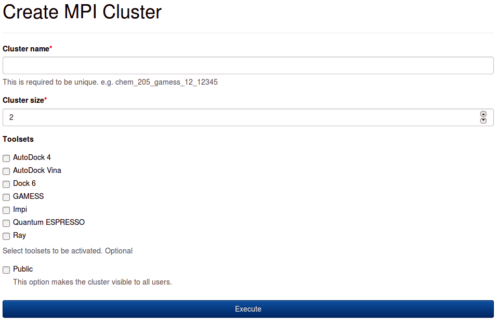
\includegraphics[scale=0.5]{./images/create_mpi.png}
				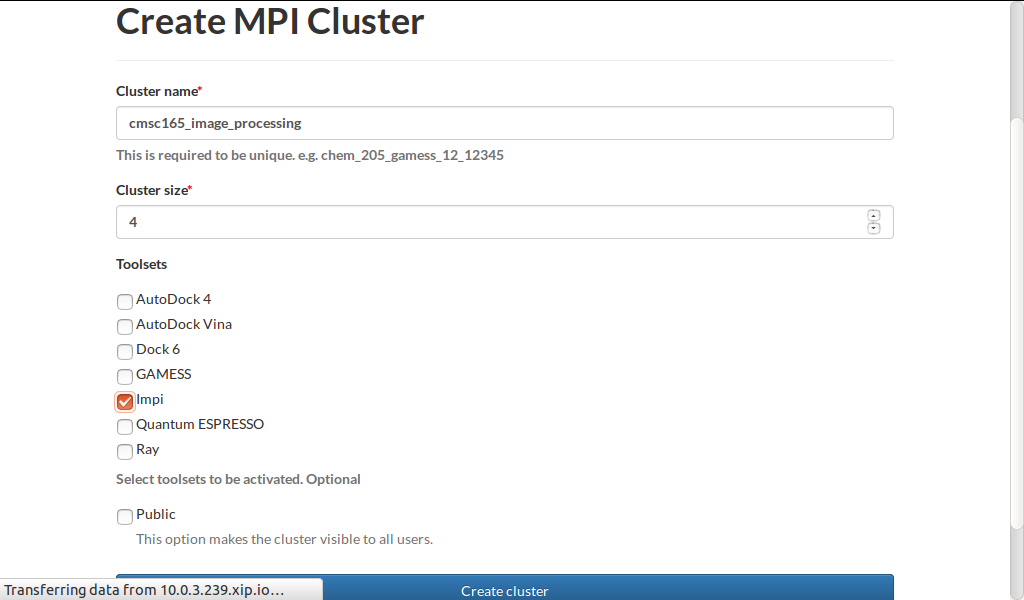
\includegraphics[scale=0.93]{./images/n_create_cluster_impi_printed.png}
				\captionof{figure}{MPI creation form}			
			\end{center}	
	
		\item The user can monitor visible public and private MPI clusters.  \newline	
		\begin{center}			
			%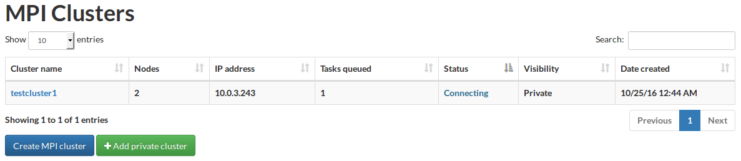
\includegraphics[scale=0.33]{./images/mpi_list_view.png}
			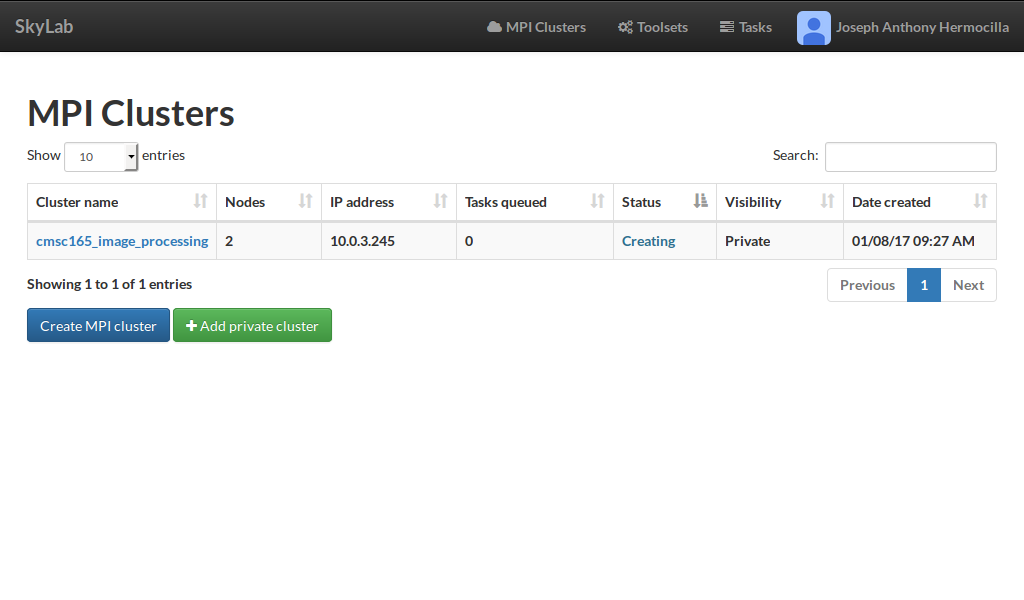
\includegraphics{./images/n_active_cluster_printed.png}
			\captionof{figure}{MPI cluster table}		
		\end{center}
		
	
		\item The user can make a private cluster visible by entering a valid share key. \newline
		\begin{center}			
			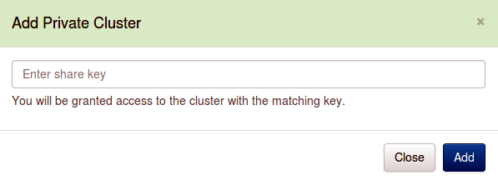
\includegraphics[scale=0.50]{./images/add_private_cluster_2.png}		
			\captionof{figure}{Add private cluster form}			
		\end{center}	
		
		\item The user can view details about a MPI cluster. If the user is the cluster's owner he has the option to delete the cluster. \newline
		\begin{center}			
			%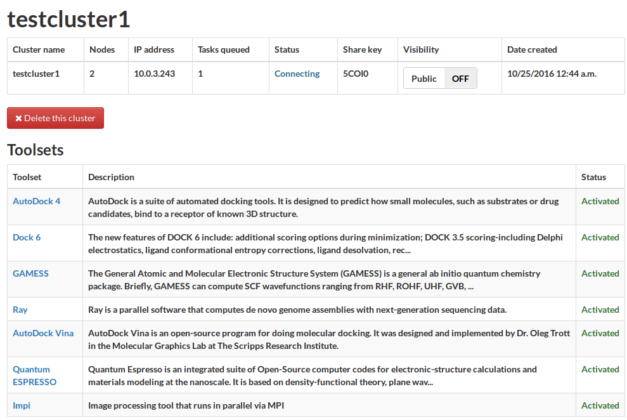
\includegraphics[scale=0.40]{./images/mpi_detail_view_2.png}			
			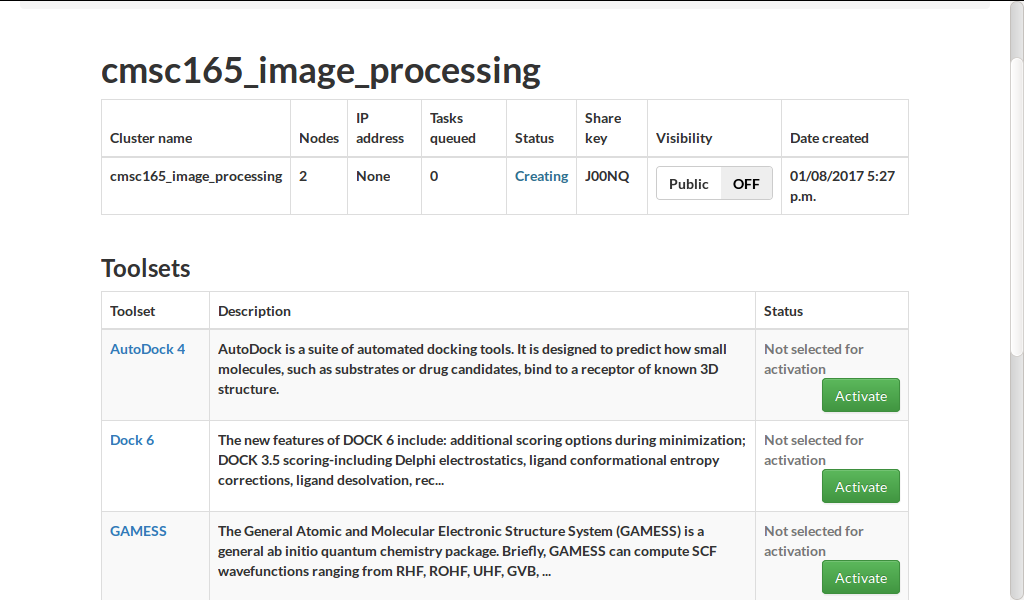
\includegraphics{./images/n_new_cluster_created_printed}
			\captionof{figure}{MPI detail view}			
		\end{center}	
		
		\item The user can select from a list which tool does he want to use. 	
		\begin{center}			
			%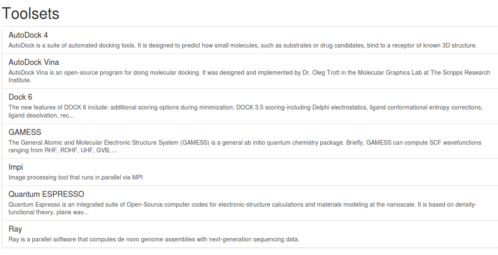
\includegraphics[scale=0.45]{./images/toolset_list_2.png}			
			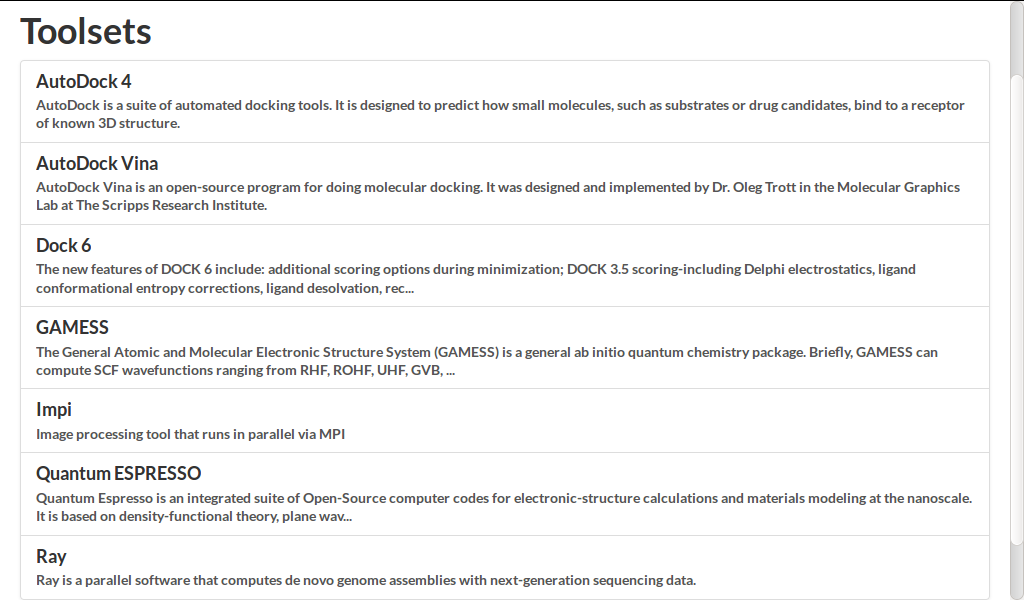
\includegraphics[scale=0.93]{./images/n_toolsets_printed.png}			
			\captionof{figure}{Toolset list view}			
		\end{center}
		
		\item The user can submit a task by filling up a tool's task creation form. \newline
		\begin{center}			
			%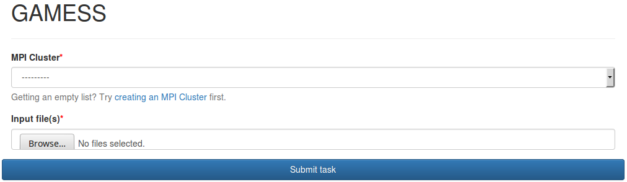
\includegraphics[scale=0.40]{./images/gamess_form_2.png}			
			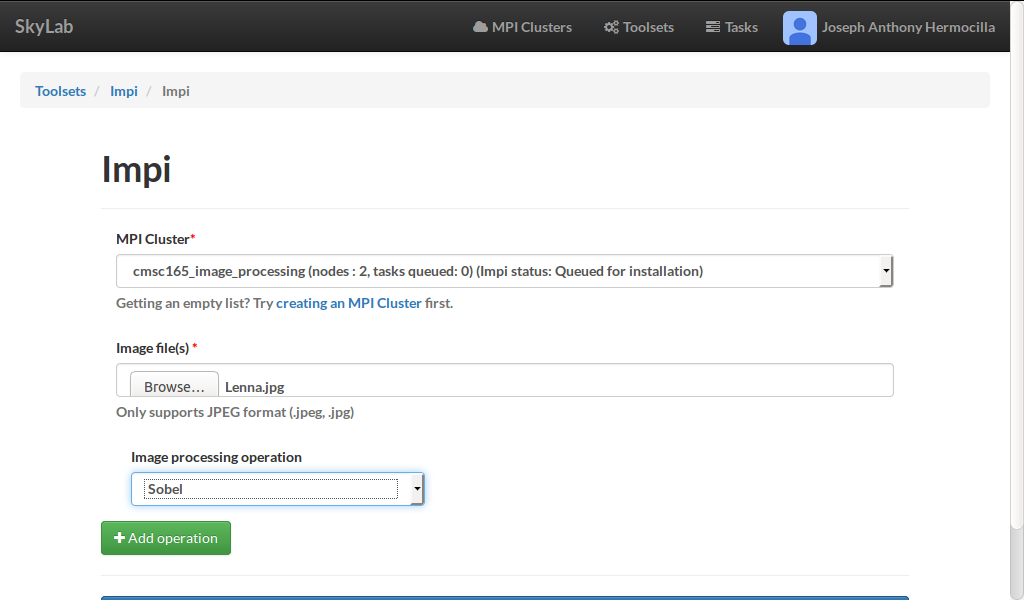
\includegraphics[scale=0.93]{./images/n_impi_parameters_printed.png}
			\captionof{figure}{GAMESS task creation form}			
		\end{center}	
		
		\item The user can monitor created tasks. \newline
		\begin{center}			
			%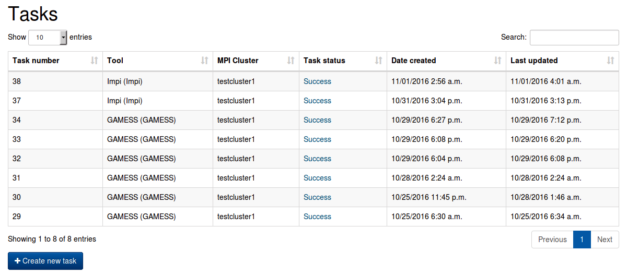
\includegraphics[scale=0.40]{./images/tasks_list_view_2.png}			
			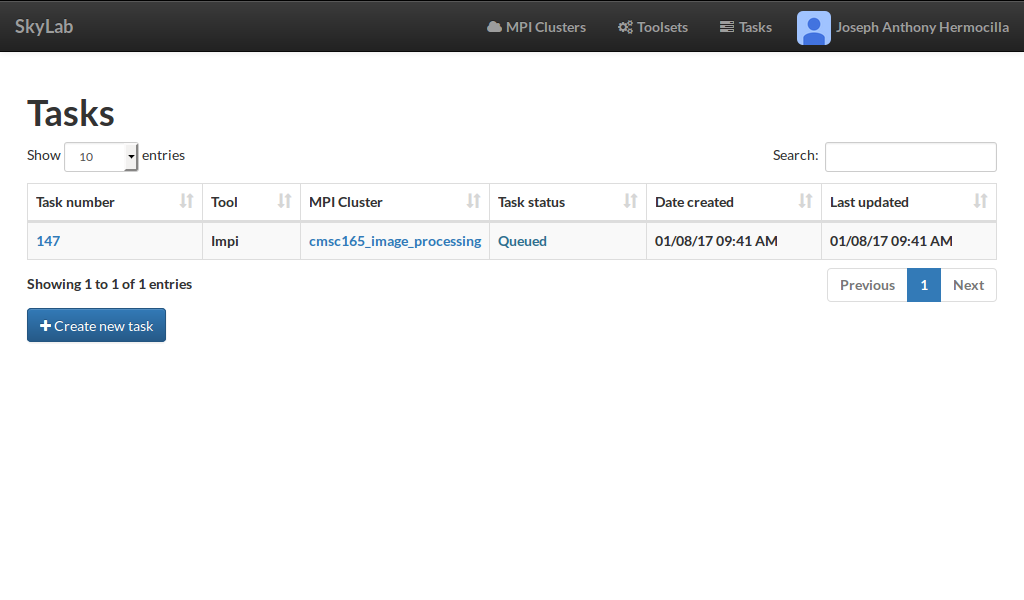
\includegraphics[scale=0.93]{./images/n_tasks_printed.png}			
			\captionof{figure}{Task table view}			
		\end{center}	
		\item The user can view results of tasks. JSmol renders the compatible output files\cite{IJCH:IJCH201300024}. \newline
		\begin{center}			
			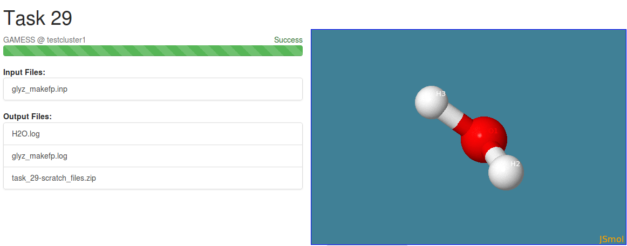
\includegraphics[scale=0.35]{./images/jsmol_detail_view_2.png}			
			\captionof{figure}{Task detail view}			
		\end{center}	

		    
		
	\end{itemize}
	
\section{Evaluation}
	\begin{center}			
			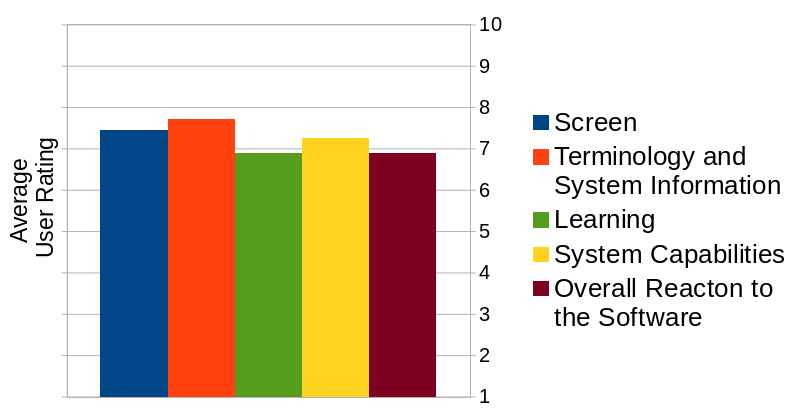
\includegraphics[scale=0.32]{./images/uat_graph.png}			
			\captionof{figure}{Results of QUIS for SkyLab}			
	\end{center}
	The system has been evaluated by 56 respondents by answering a survey based on Questionnaire for User Interface Satisfaction (QUIS) \cite{chin1988development}. Respondents are students who are unfamiliar with both HPC tools and the concept of MPI systems.  Respondents are asked to test features of SkyLab by following a set of instructions and using input files provided. On the average, the users rated their overall experience with SkyLab to 6.9/10. The users listed the simplicity of the user interface to be the most positive aspect of the system while the slow speed of task processing is said to be the most negative. Majority of the tools supported by SkyLab have inherently long processing time which is not known to the respondents. The system does not focus on optimizing the said tools to achieve better performance but rather it focuses on simplifying the user's task submission process. 

\section{Related Work}
Ganglia is a system designed to monitor high performance computing systems. It uses a hierarchical model in managing the system of clusters. It uses optimized data structures and communication algorithms to achieve scalability with high concurrency. It is claimed to be used by over 500 clusters around the world. This implies that the system is tested and trusted to be used for real-world applications\cite{1395654820040701}.
	    
One of the main inspirations for developing SkyLab is the Yabi system. It provides a web interface with support for workflow environments with focus on introducing HPC applications to non-technical audience. Users can create and reuse workflows, and manage large amounts of data while system administrators can configure tools via the web interface as well. It is currently in use by multiple institutions, and is maintained as an open-source project\cite{7411021620120101}.	    	    
	    
Another related project is Web Interface for mpiBLAST (WImpiBLAST). It supports mpiBLAST, a parallel implementation of Basic Local Alignment Search Tool (BLAST). BLAST is a software used for sequence homology similarity search in large databases of gene sequences. mpiBLAST can utilize HPC clusters to achieve faster computing speeds but it requires knowledge in using MPI commands to benefit from its advantages. WImpiBLAST addresses this problem by providing the user a web interface to simplify the steps to use mpiBLAST\cite{9686120720140601}.   
	
\section{Conclusion and Future Work}
The system created allows users to manage MPI clusters and submit tasks without the need for technical expertise in scripting. This makes the advantages of HPC available to non-technical users. This is achieved by parsing form inputs to generate commands for task execution. Task files can be download from the server and output files are displayed with the help of JSmol\cite{IJCH:IJCH201300024}. The system is also configured to install tool sets found in the modules folder making it possible to accommodate additional tools. Based on the user acceptance test conducted, the users found the system to be acceptable in terms of the criteria provided, in general. 

The system achieved its main objectives but its features can still be improved and additional features can be introduced. Improved input parameter checking and error handling will make the system more robust. There are still use cases of tools that are yet to be supported. Input file generation can make the process more interactive and more customizable.  Workflow design support will enable users to run complex tasks. Support for custom MPI programs will make it easier for developers to utilize the system as a test environment. Task scheduling and resource management algorithms can be used to efficiently handle resource-intensive or time consuming tasks. For example, a cluster can borrow resources from idle clusters. These recommendations will provide the users a better experience in using the system for academic and research purposes. 

% APPENDICES
%\appendices

%\section{Proof of the First Zonklar Equation}
%Appendix one text goes here...

%\section{}
%Appendix two (without title) text goes here...

% ACKNOWLEDGMENT
\section*{Acknowledgment}
This work is supported by the Philippine Department of Science and Technology Accelerated Science and Technology Human Resource Development Program.
%Many thanks to...
% BIBLIOGRAPHY
% \nocite{*}

% BIOGRAPHY
%\begin{biography}[{
\includegraphics{./yourPicture.eps}}]{Student M. Name}
%Biography text here...
%\end{biography}



